\documentclass[a4 paper, 11 pt, twocolumn]{article}

\usepackage[left=0.5in, right=0.5in, top=1in, bottom=1in]{geometry}
\usepackage{fancyhdr}
\usepackage{graphicx}
\usepackage{amsthm}
\usepackage{amsmath}
\usepackage{amssymb}
\usepackage{multirow}
\usepackage{graphicx}

\begin{document}
\begin{titlepage}
\begin{center}
\textsc{\huge Regression Homework 3} \\ [0.5cm]
\textsc{\huge Monthly Rent in Manhattan}\\ [1.5cm]
\textsc{\large Janet Ye: jy1151} \\
\vfill
{\large \today}
\end{center}
\end{titlepage}

\section{Introduction}
Manhattan is one of the most populated cities in the world. It is known for its expensive real estate prices. In this analysis, one explores the monthly rent prices of Manhattan in relations to several quality measures, including numbers of bedrooms, bathrooms, square feet, crime rate in the precinct, and whether the building has a doorman.
\section{The Data}
The data is obtained in mid-March from StreetEasy, a popular apartment rental website. I skipped any apartments with incomplete information, e.g. I omitted apartments without square feet information. I manually recorded 200 listings in all Manhattan precincts, with their rent prices and quality measures. All apartments are unfurnished and had been posted on the website for less than a week at the time of data collection.

Number of bedrooms, number of bathrooms, square feet of the apartment are all self-explanatory. Crime rate is number of crimes per 1,000 residents in February 2014 obtained from http://maps.nyc.gov/crime/. The variable doorman is an indicator variable, 1 if the building has a doorman (virtual doorman does not count), 0 if not.

One begins with a summary of our data set.
\begin{center}
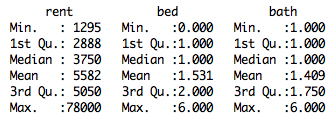
\includegraphics[scale=0.7]{sum1}
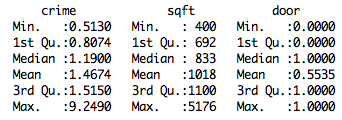
\includegraphics[scale=0.7]{sum2}
\end{center}
For the variable rent price, the median is \$3,750 and the mean is \$5,582. This indicates that rent price is skewed right. Indeed, the most expensive rent in our sample is a 3831 square-feet apartment in Upper West Side (15 Central Park West) that oversees the Central Park, which very well brings up the mean.

Our sample includes from studio apartments to 6-bedroom apartments with six bathrooms. Crime rate spans from 0.5130 per 1,000 residents to an unbelievably high of 9.2490 per 1,000 residents in Midtown south. Similar to rent price, number of square feet is also skewed right, with median 833 and mean 1018.

Is rent price related to quality measures? One can look at the scatterplots of rent price against number of bedrooms, number of bathrooms, crime rate, and number of square feet. One omits the scatterplot of rent price against the indicator variable doorman.
\begin{center}
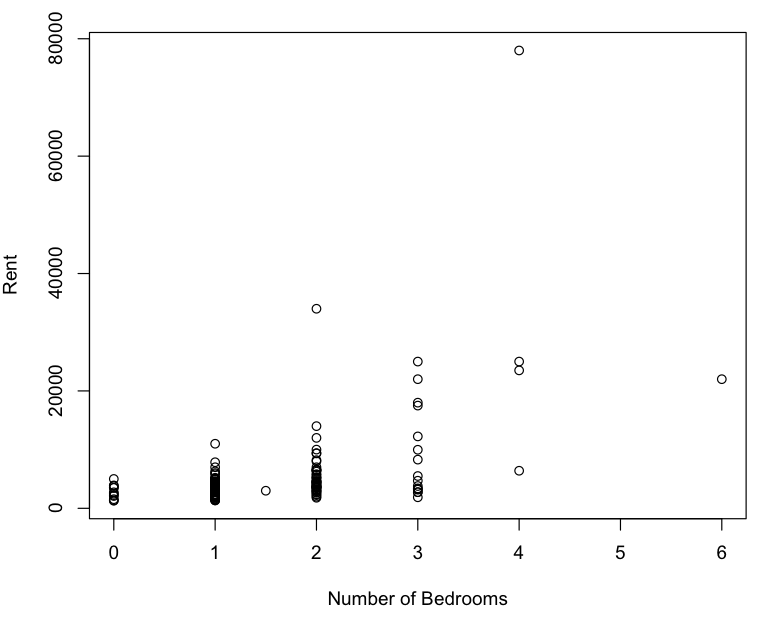
\includegraphics[scale=0.3]{scatter1}
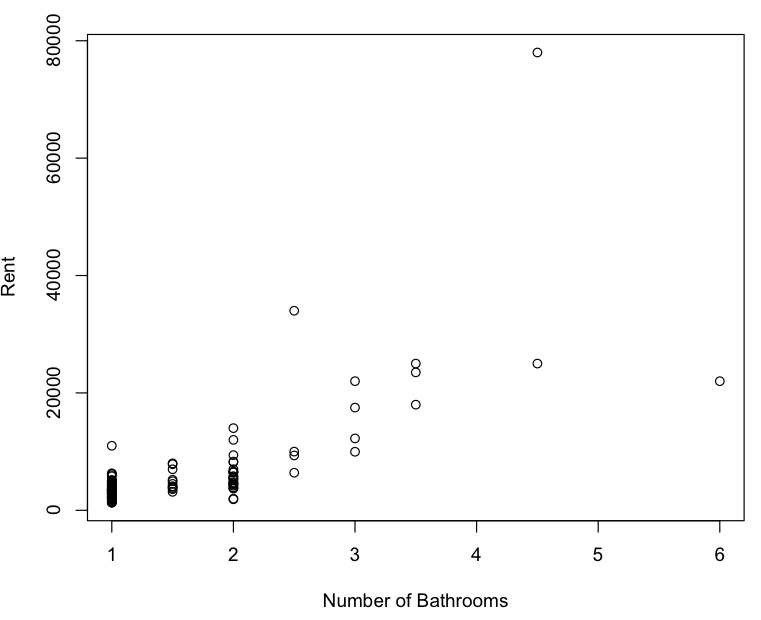
\includegraphics[scale=0.3]{scatter2}
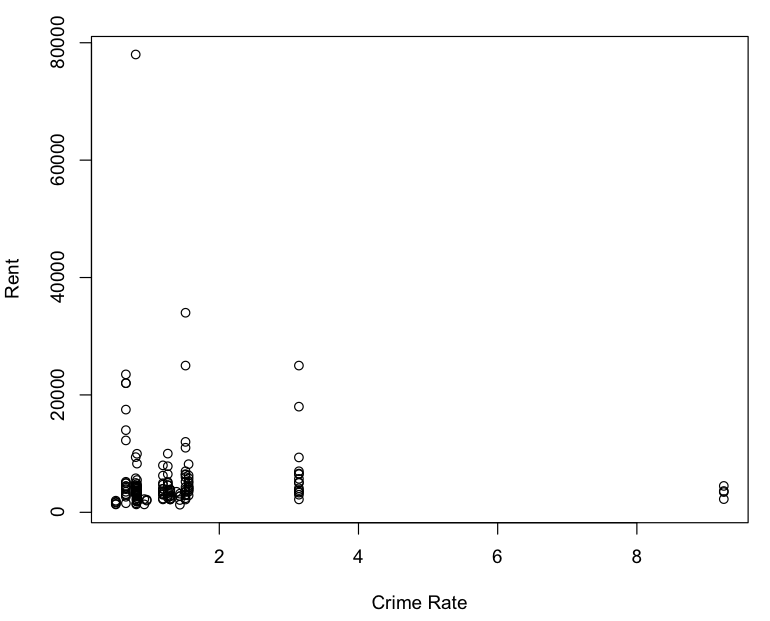
\includegraphics[scale=0.3]{scatter3}
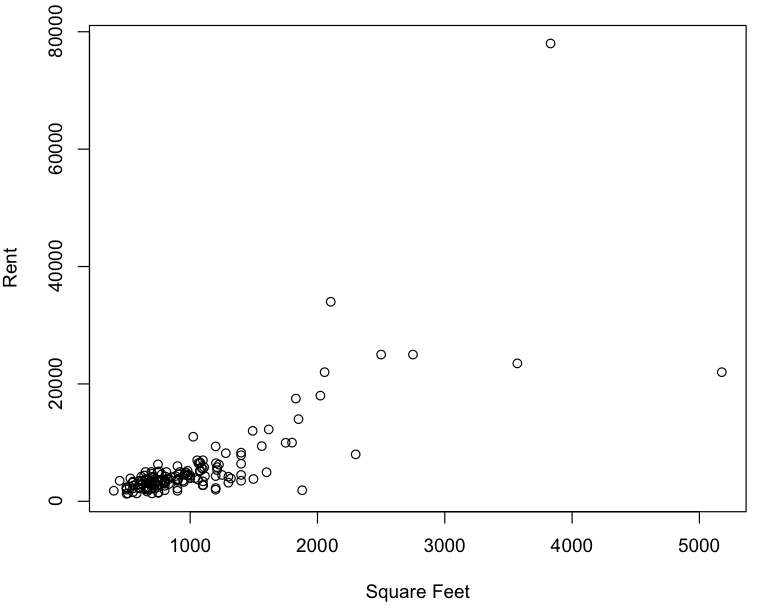
\includegraphics[scale=0.3]{scatter4}
\end{center}
Crime rate versus rent has the weakest relationship. One would expect apartments in low crime rate precincts have higher rent. The negative relationship is not clear in the scatterplot. In the scatter plot square feet versus rent, there are some points that are of concern. Namely, the apartment in Upper West Side that oversees Central Park has unusually high rent, close to 80,000. The point to the far right is a 5,176-square feet townhouse in Upper East Side (157 E82). There are some other alarming points, and we will keep them in mind as we look at the multiple regression.

\section{Multiple Regression}
Here is the regression output.
\begin{center}
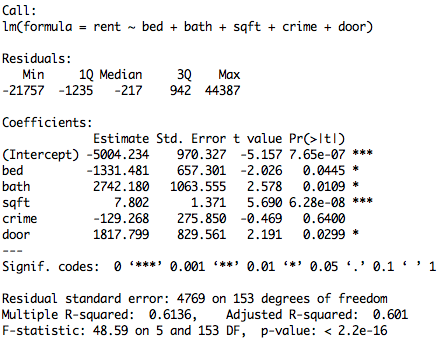
\includegraphics[scale=0.55]{mr1}
\end{center}
Multicollinearity is not a problem, since $VIF < 10$.
\begin{center}
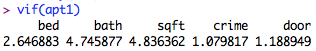
\includegraphics[scale=0.6]{vif}
\end{center}
The multiple regression equation is
\begin{align*}
\text{Rent } &= -5004.234 -1331.481\times \text{Number of Bedroom} \\
&+ 2742.18\times \text{Number of Bathroom} + 7.802 \times \\ &\text{Number of Square Feet} -129.268\times \text{Crime Rate} \\&+ 1817.799\times \text{Doorman}
\end{align*}
The intersection is meaningless, as no apartment has 0 square feet (with no bedroom, bathroom, or doorman in a perfectly safe precinct).

The coefficient for bedroom is counterintuitive. It means holding all else constant, an apartment with one more bedroom is associated with \$1331.481 decrease in monthly rent. This presents an arbitrage opportunity, meaning if two apartments having the same area and other quality measures, the one with an extra bedroom would be cheaper. For example, we consider two apartments in Midtown North. 1 Central Park South is a 695 square feet studio apartment, with a bathroom and doormen. The rent for this apartment is \$5,000. On the other hand, 550 W54 is a one-bedroom, one-bathroom apartment with 650 square feet and doormen in Midtown North. It costs \$3,800.

The model also suggests that if holding all else constant, having an extra bathroom is associated with \$2742.18 increase in rent. One extra square foot is associated with \$7.802 increase in rent holding all else constant. One more crime per 1,000 residents in a particular precinct is associated with \$129.268 decrease in rent, holding all else constant. An apartment with doormen is associated with \$1817.799 more in rent compare an identical apartment without doormen.

As previously observed, the variable "Crime Rate" does not add any predictive power for price of the rent. Its t-statistic is -0.469, with a p-value of 0.64, which is above $\alpha=$ 0.5.

A residual standard error of 4769 implies that this model could be used to predict the rent price to within roughly $\pm \$9,538$, 95\% of the time.

The regression is moderate to strong. A $R$-squared of 61.36\% tells us that 61.36\% of the variability in rent prices can be explained by the linear relationship with number of bedrooms, number of bathrooms, square feet, crime rate, and whether the apartment has a doorman.

\section{Regression Diagnostics}
\begin{center}
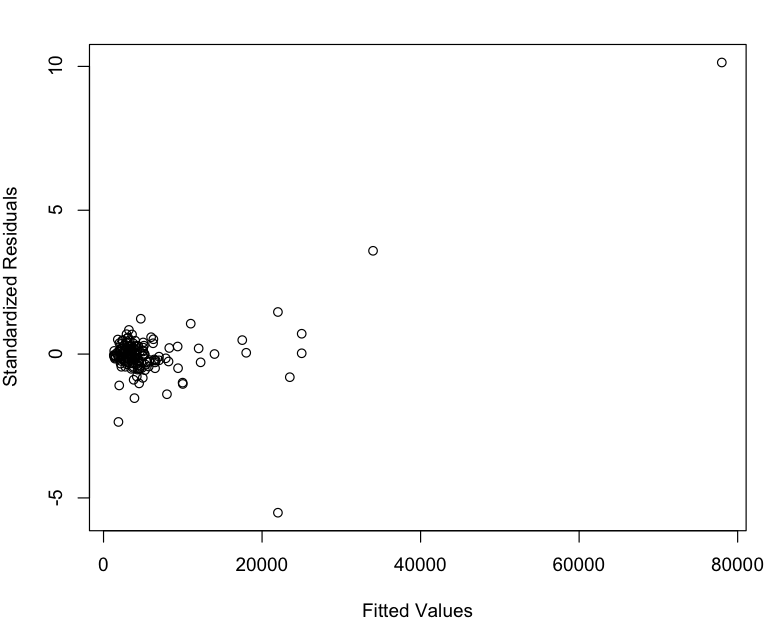
\includegraphics[scale=0.25]{residual}
\end{center}
Looking at the standardized residuals versus fitted values plot, we expect 95 percent of the apartments lie within $\pm 2.5$ standardized residuals. There are three points that should be investigated as outliers. As we suspected, the one with unusually low rent is observation 96, 157 E82 -- the townhouse in Upper East Side. The townhouse has 5,178 square feet with six bedrooms and six bathrooms, and 0.6578 crimes per 1,000 residents, but no doorman. The rent is \$22,000, which is unusually low comparing to similar apartments in Manhattan. Perhaps this unusually low rent is because the residence is a townhouse, and has no management to maintain the place.

The apartment in the middle of the plot has a standardized residual of almost 4. This is observation 59, 212 W18. The apartment has 2 bedrooms, 2.5 bathrooms, 2,104 square feet, with 1.515 crimes per 1,000 residents and doormen. The rent is \$34,000.

Finally, the apartment to the far right of the plot with absurdly high standardized residuals of 10 is 15 Central Park West, another observation we noted before. The residual plot agrees with our intuition, and the high rent of this apartment is truly unusual.

\begin{center}
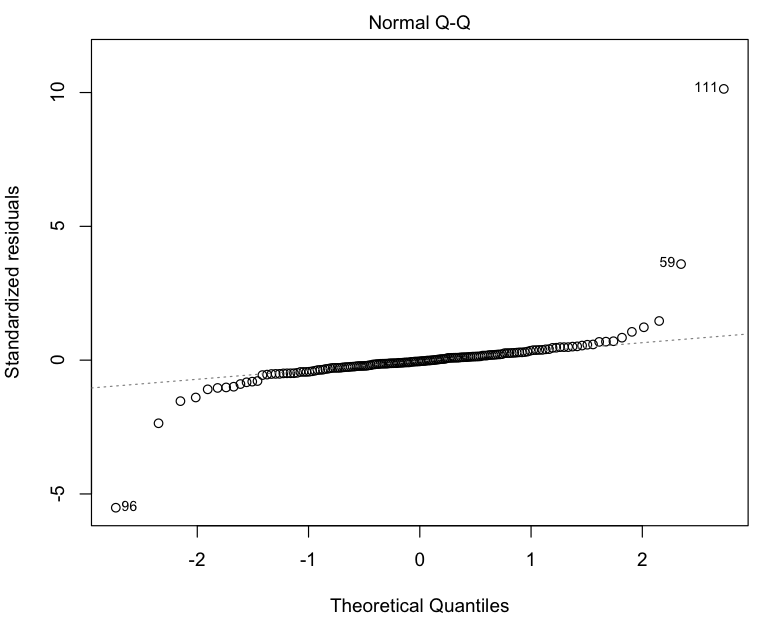
\includegraphics[scale=0.3]{QQ}
\end{center}
The QQ-plot also marks the three unusual points noted above. The following plot shows Cook's distance in dotted lines. Cook's distance picks up influential points.
\begin{center}
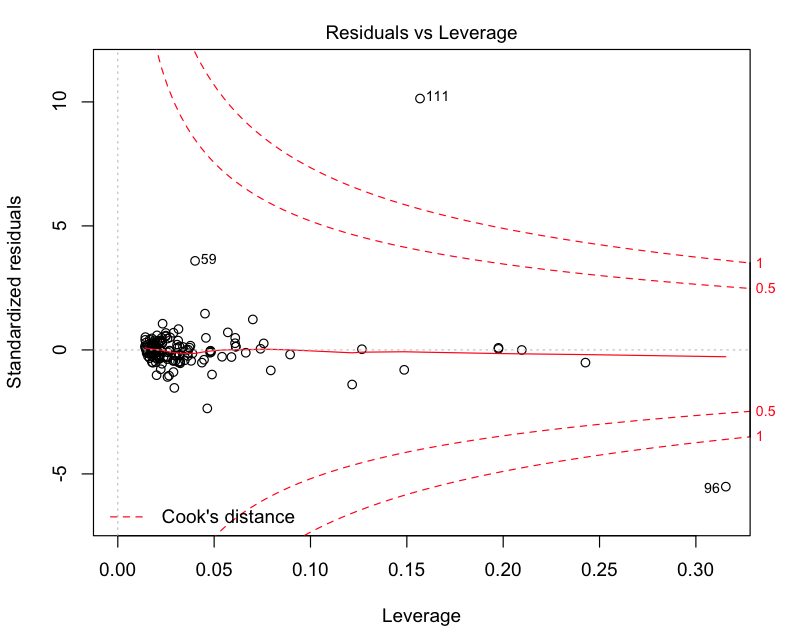
\includegraphics[scale=0.3]{CooksD}
\end{center}
Observations 96 and and 111 are outside the $D=1$ range. Both observations are noted above.

The graph also shows leverage on the horizontal axis. Leverage is a good measure to pick up leverage points. A good guideline for what constitutes a large leverage value is $2.5\left(\frac{p+1}{n}\right) = 2.5 \left(\frac{5+1}{160} \right) = 0.09375$. We see that there are six points that are leverage points, being at the far right of the horizontal axis. Again, observations 111 and 96 are potential ``bad'' leverage points, as they are outliers and have leverage greater than 0.09375.

By looking at the standardized residuals, QQ plot, leverage values, and Cook's distance, we have observed three problematic points, which are observations 59, 111, and 96. We proceed to remove these outliers and run the regression again.

\section{The Second Pass}
After removing the three outliers, we essentially have a new data set. We begin with a summary.
\begin{center}
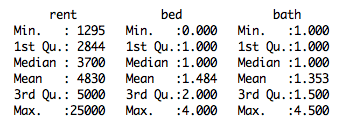
\includegraphics[scale=0.7]{suma}
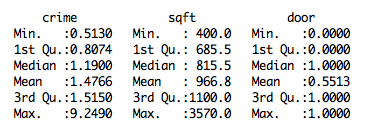
\includegraphics[scale=0.68]{sumb}
\end{center}
Notice the mean decreases from \$5,582 to \$4,830 after removing the points. The median is \$3,700, so rent is still skewed right. The maximum number of bedrooms is now 4; the maximum amount of bathrooms is 4.5. Crime rate remains the same, with minimum of 0.5130 per 1,000 residents and maximum of 9.249 per 1,000 residents. The area of the apartments range from 400 square feet to 3570 square feet.

We again look at the scatterplots of rent price against number of bedrooms, number of bathrooms, crime rate, and number of square feet. We omit the scatterplot of rent price against the indicator variable doorman, as it is not meaningful.
\begin{center}
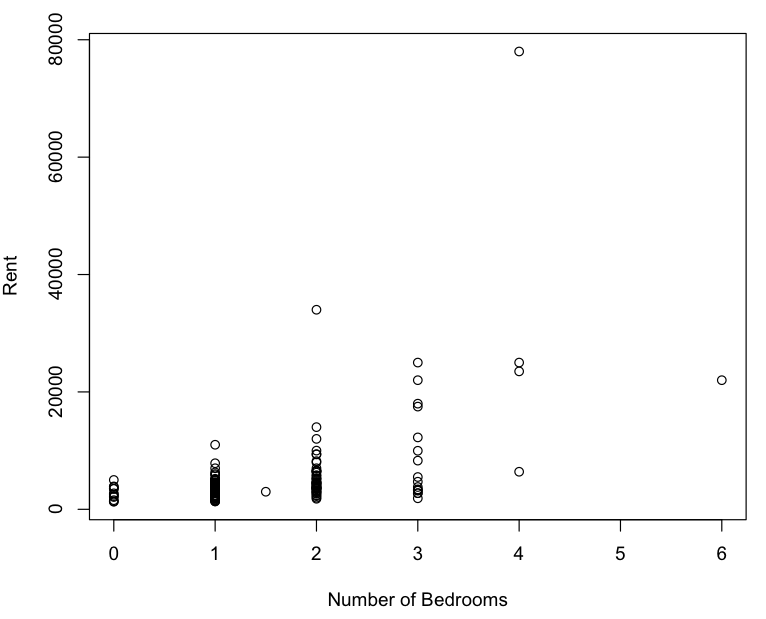
\includegraphics[scale=0.35]{scattera}
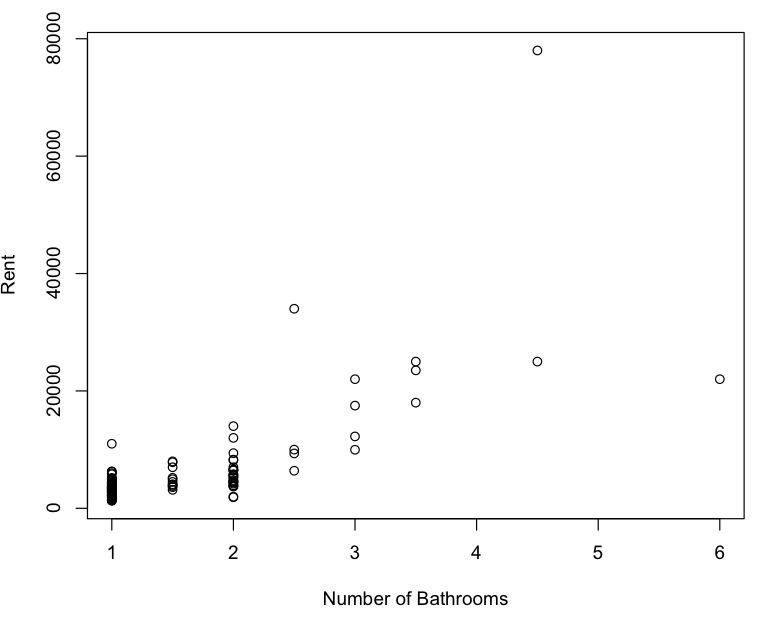
\includegraphics[scale=0.35]{scatterb}
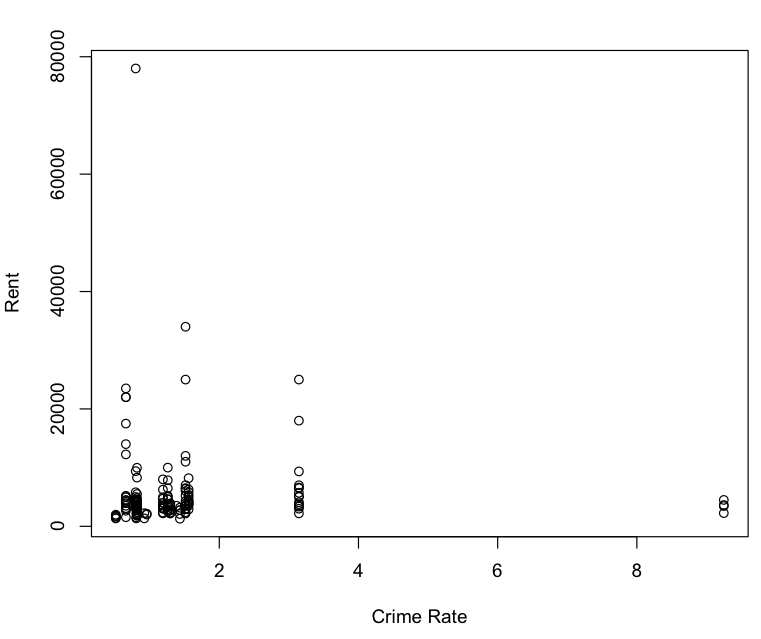
\includegraphics[scale=0.35]{scatterc}
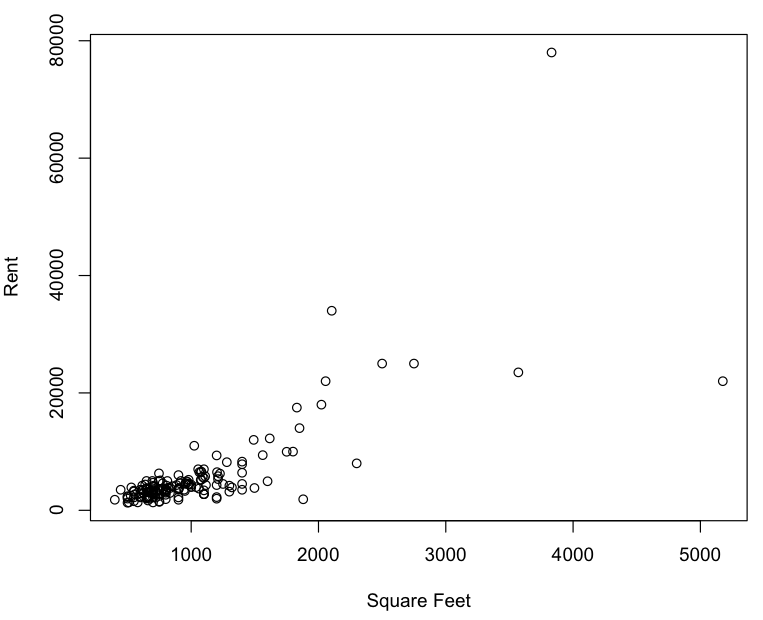
\includegraphics[scale=0.35]{scatterd}
\end{center}
Again, we see that crime rate has the weakest relationship. The negative relationship is not clear. In the scatterplot of rent versus square feet, there is a point with unusually high rent. It is observation 111, 124 W60, a 618 square-feet one-bed, one-bath apartment in Upper East Side (crime rate 0.7990 per 1,000 residents) with doormen, pricing at \$3,450. After examining the original advertisement, there is no additional information that suggests this apartment is special in some ways, resulting in such a high rent. This is a potential outlier that one should keep in mind of.

\section{Multiple Regression 2}
Below is the regression output.
\begin{center}
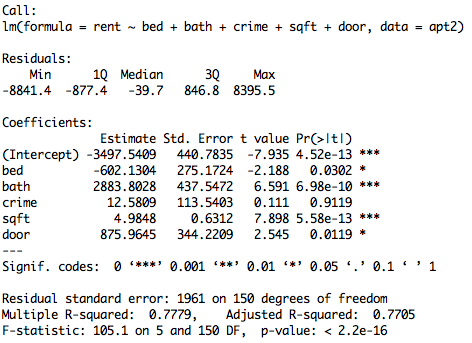
\includegraphics[scale=0.55]{mr2}
\end{center}
The multiple regression equation is,
\begin{align*}
\text{Rent } &= -3497.5409 -602.1304 \times \text{Number of Bedrooms} \\
&+ 2883.8028 \times \text{Number of Bathrooms} \\
&+12.5809 \times \text{Crime Rate} + 4.9848 \times \text{Square Feet} \\
& +875.9645 \times \text{Doorman}
\end{align*}
A significant change here is that the coefficient for Crime is now positive. Holding all else constant, one more crime per 1,000 residents is associated with \$12.5809 increase in rent. Looking at its t-statistic, we see that crime has a p-value of 0.9119, thus again does not add predictive power to price of the rent.

All other variables are significant using $\alpha =0.5$. We proceed to interpret the coefficients. The intercept is meaningless, for reason explained previously. Holding all else constant, one more bedroom is associated with -\$602.1304 in rent. One more bathroom is associated with \$2883.8028 increase in rent holding all else constant. One square foot increase in apartment size is associated with \$4.9848 increase holding all else constant. An apartment with doormen is associated with \$875.9645 more in rent compare to an identical apartment with doormen.

Notice that $R-$squared pleasantly increases to 77.79\% after removing those three outliers, meaning 77.79\% of the variability in price of rent is explained by the linear relationship with variables number of bedrooms, number of bathrooms, crime rate, size of the apartment(square feet), and whether the apartment has doormen.

Notice also that the residual standard error (albeit still big) reduces dramatically to 1961. This model could be used to predict the rent price to within roughly $\pm 3922$ 95\% of the time.

Also, $VIF<10$ is not a problem.
\begin{center}
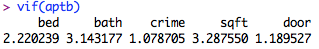
\includegraphics[scale=0.6]{vif2}
\end{center}

\section{Regression Diagnostic}
\begin{center}
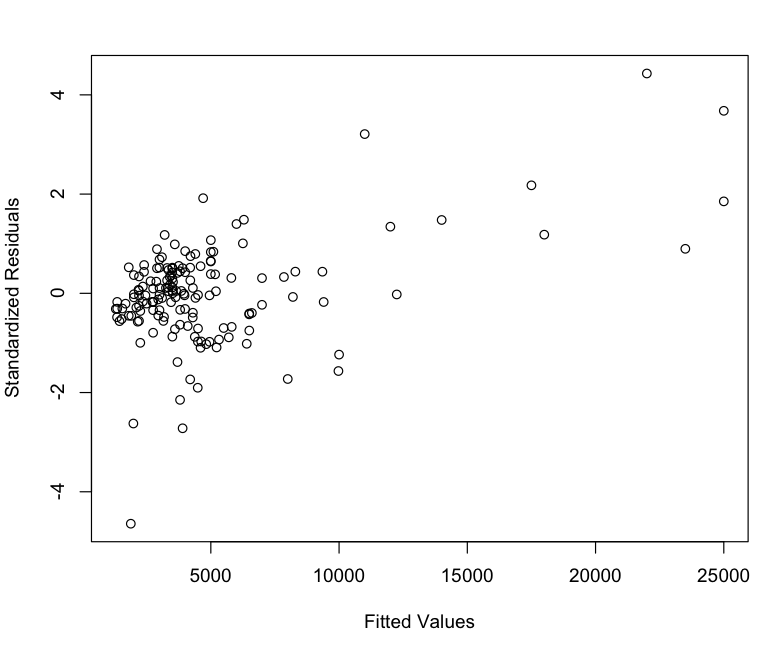
\includegraphics[scale=0.3]{residual2}
\end{center}
One can make two observations from this standardized residuals versus fitted values plot. One, data are mostly concentrated with rent less than \$10,000. Almost all of these data have standardized residuals within $\pm 2.5$. Our model does not do so well with apartments on the right side of the residual plot -- the standardized residuals are strictly higher. Therefore, our model tends to underpredict in these cases.

We include the same plot with tagged points to study potential outliers.
\begin{center}
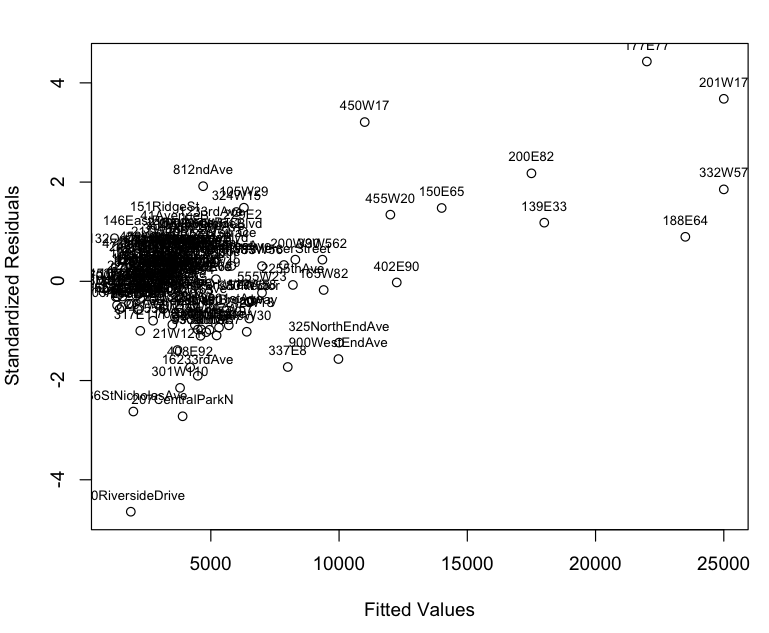
\includegraphics[scale=0.3]{residualbrush}
\end{center}
Second observation is that there are three points with standardized residuals greater than $+$2.5, which are 450 W17(observation 57), 177 E77(observation 86), and 201 W17(Observation 60). 450 W17 has rent price of \$11,000, one bedroom, one bathroom, 1024 square feet with doormen and crime rate of 1.515 per 1,000 residents. 177 E77 has rent price of \$3950, one bedroom, one bathroom, 1038 square feet with no doormen and crime rate of 0.6578. 201 W17 has rent price of \$6,500, two bedrooms, two bathrooms, 1203 square feet with doormen and crime rate of 0.7990. Examining the data, one sees that there is nothing special about these apartments.

290 Riverside Drive (observation 87) has a standardized residual of -4.5, so the model overpredicts its rent price. The apartment rents for \$3,750, two bedroom, one bathroom, 900 square feet, with no doormen and a crime rate of 0.8172 per 1,000 residents. This is because uptown real-estate is naturally cheaper than other neighborhoods. However, our model seems to do fine with other uptown real estates. This is a sign that our model lacks some other predictors.

\begin{center}
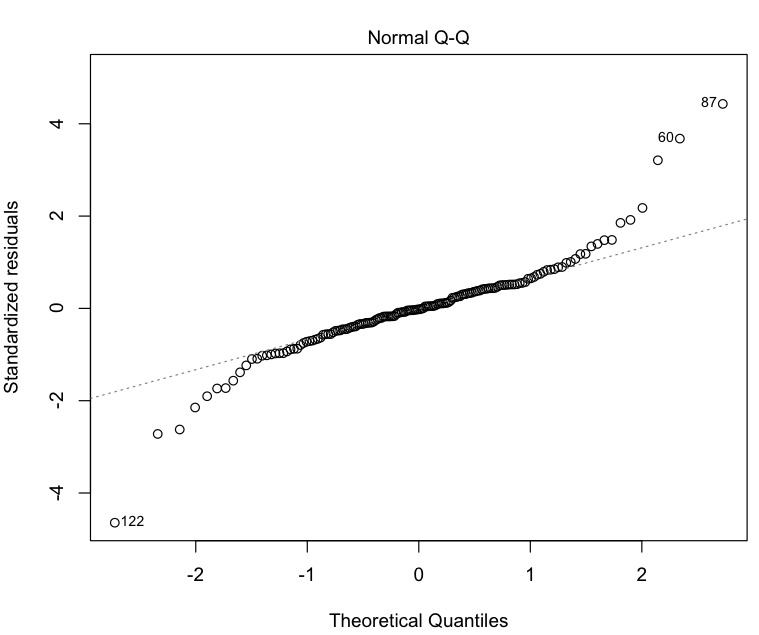
\includegraphics[scale=0.3]{QQ2}
\end{center}
Three points deviate from the line in QQ plot, which are 201 W17(observation 60) examined above, 177 E77 (observation 87), and 290RiversideDrive (observation 87) from above.

\begin{center}
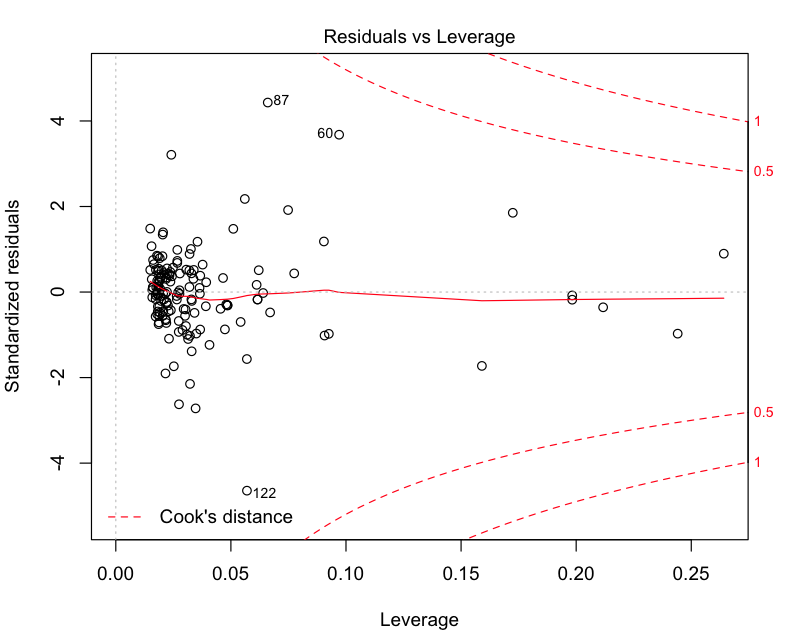
\includegraphics[scale=0.3]{CooksD2}
\end{center}
Cook's Distance measures influential points. All points have Cook's D less than 1. The appropriate guideline for leverage value is $2.5\left(\frac{p+1}{n}\right) = 2.5\left(\frac{5+1}{156}\right) = 0.9615.$ There are six points again to the right of this desired value, and are potential leverage points.

\section{Third Pass}
From previous two multiple regression analysis, one sees that crime rate is not a particularly useful predictor. Hence, we will conduct a multiple regression using \textit{original} data set with only four predictors, number of bedroom, number of bathroom, square feet for size, and indicator variable doorman.

Below is the regression output.
\begin{center}
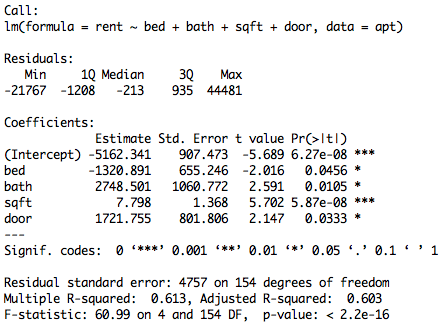
\includegraphics[scale=0.5]{mr3}
\end{center}
The equation does change much.
\begin{align*}
\text{Rent } &= -5162.341 -1320.891\times \text{Number of Bedroom} \\
&+ 2748.501\times \text{Number of Bathroom} + 7.798 \times \\ &\text{Number of Square Feet} +1721.755\times \text{Doorman}
\end{align*}
$R$-squared remains the same compare to the first pass at 61.3\%.
\begin{center}
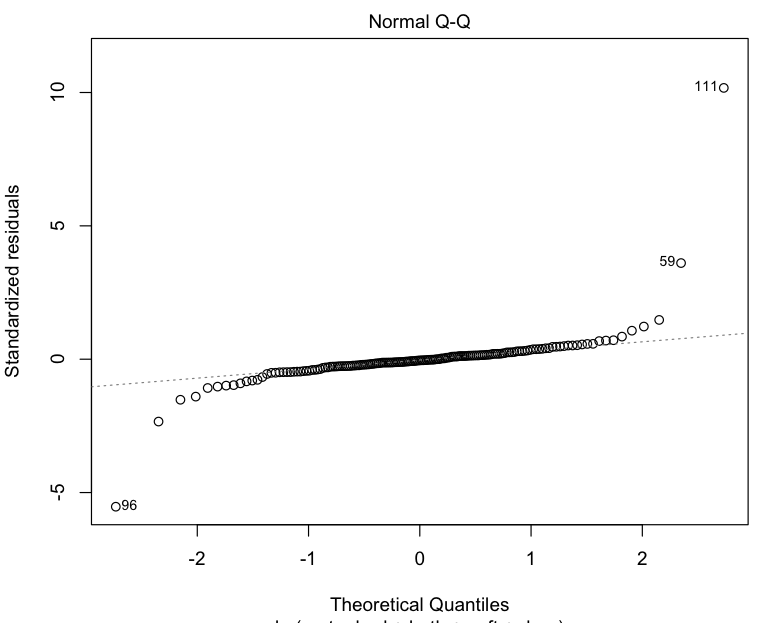
\includegraphics[scale=0.3]{QQ3}
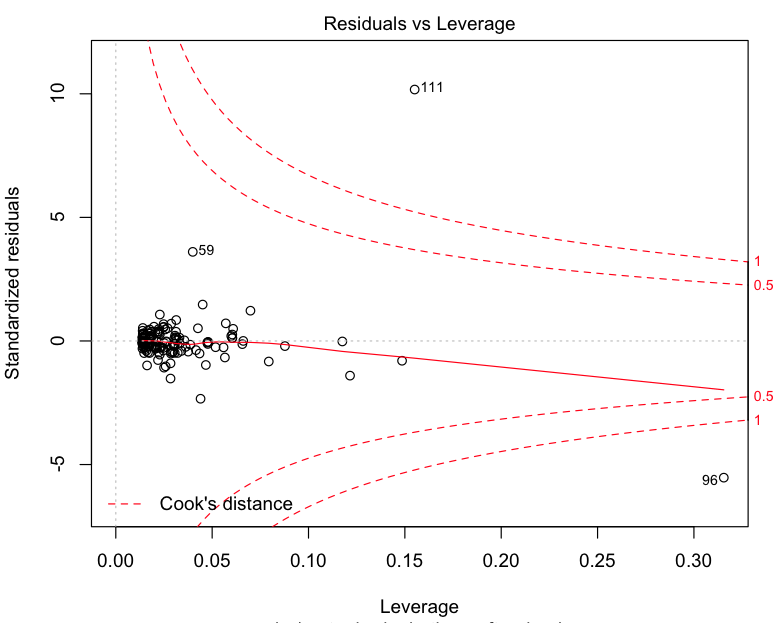
\includegraphics[scale=0.3]{CooksD3}
\end{center}
Residual diagnostics pick up the same three outliers as first pass, 212 W18(observation 59), 157 E82 the townhouse (observation 96), 15 Central Park West (observation 111). We will remove these outliers and run the model again using only four variables.
\section{The Final Pass}
\begin{center}
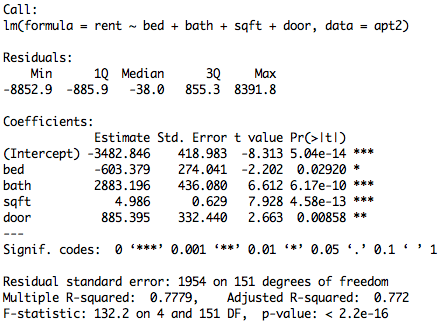
\includegraphics[scale=0.5]{mr4}
\end{center}
Excluding the outliers, the multiple regression equation is now,
\begin{align*}
\text{Rent } &= -3482.846 -603.379\times \text{Number of Bedroom} \\
&+ 2883.196\times \text{Number of Bathroom} + 4.9866 \times \\ &\text{Number of Square Feet} +885.395\times \text{Doorman}
\end{align*}
All predictors are significant at $\alpha = 0.05$ level. $R$-squared is 77.79\%, same as second pass. This is a sign that crime rate does not add any value to our model, thus one should always opt in for the simpler model.
\begin{center}
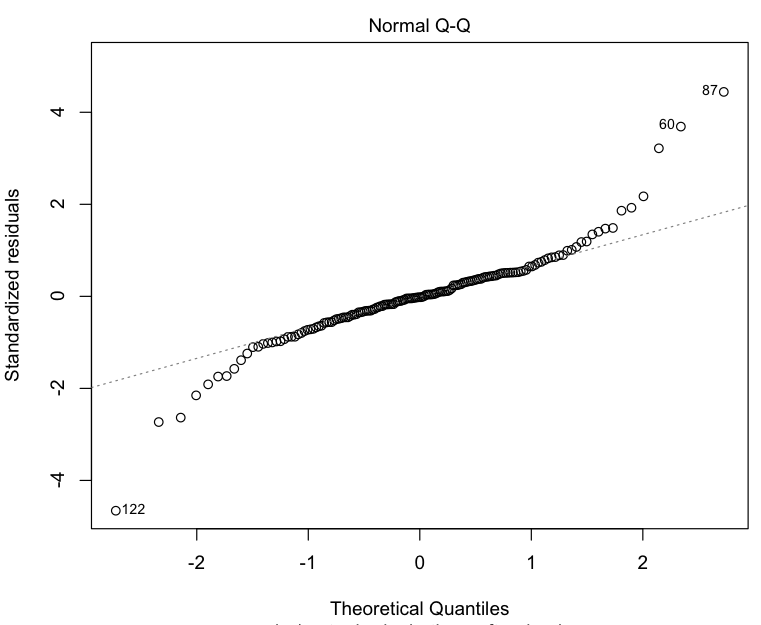
\includegraphics[scale=0.3]{QQ4}
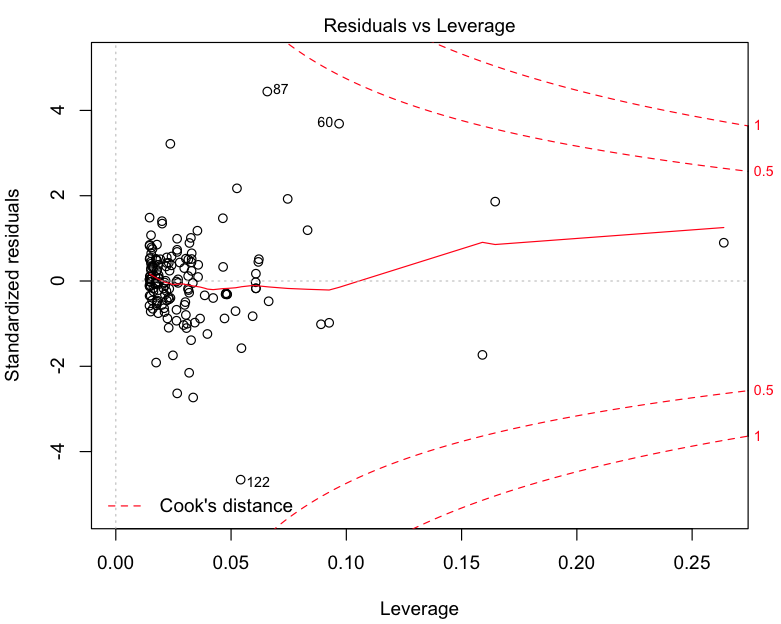
\includegraphics[scale=0.3]{CooksD4}
\end{center}
Cook's Distance looks fine; all points are within 1. Standardized residuals and QQ plot pick up three problematic points, 247 W87(observation 122), 56 7th Ave (observation 60), and 151 E85(observation 87).

Our model does okay, and there is no point to remove these outliers. We proceed to test our models using 50 holdout sample points. They are collected the same way as original data set.
\section{Holdout Data}
A list of new data used is provided in the appendix. Here's a quick summary.
\begin{center}
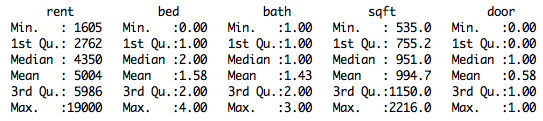
\includegraphics[scale=0.45]{sum}
\end{center}
Using the final pass model, we have the following predictions and residuals.
\begin{center}
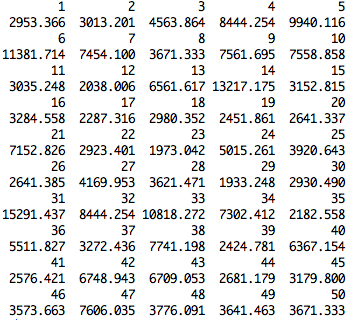
\includegraphics[scale=0.5]{pred}
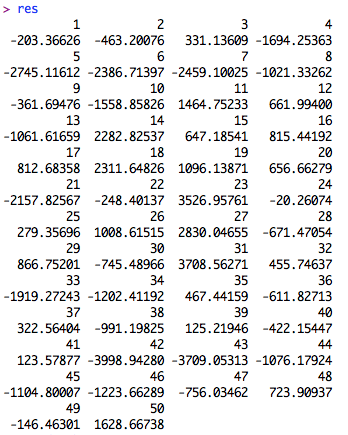
\includegraphics[scale=0.5]{res}
\end{center}
These lists of output are not particularly exciting. Here is a plot of the residuals, i.e., observed value minus predicted values.
\begin{center}
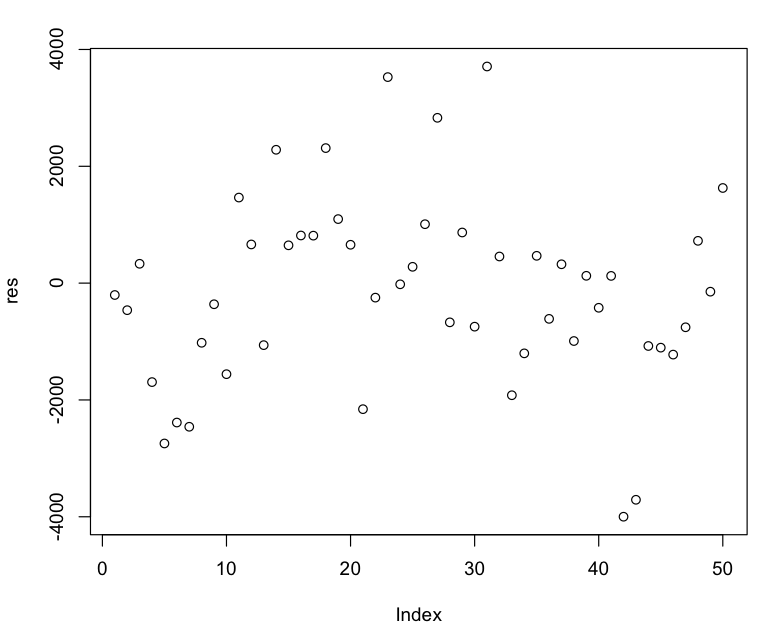
\includegraphics[scale=0.3]{resplot}
\end{center}
Notice that all data have residuals $\pm 4000$. The residual standard error for the final pass is 1954, so it is reasonable to expect the model to predict data within $\pm \$3908$ 95\% of the time. The new data demonstrates that the final pass model does reasonably well (although it is always ideal to reduce the residual standard error).
\section{Conclusion}
In the second pass, the standardized residuals versus fitted values plot shows that our model tends to do well with apartments with predicted rent less than \$10,000. The model tends to underpredict for some apartments at the right side of the residual plot. These are mostly uptown apartments.

This brings to the question of variable selections. Surely, there are other valid potential predictors, such as the popularity of a particular precinct/neighborhood, if there is laundry room in the building, the age of the apartment building, convenience access to transportation, etc. One must recognize that it is costly to obtain these pieces of information as part of data collection, or it may be simply that the owner/broker does not reveal all of our desired quality measures on StreetEasy. Even if we have information for all these extra variables, one should not solely rely on the computing power of software to determine which quality measures one should include in the model.

On the same note, through this analysis we notice that the variable crime rate is an unnecessary. It adds no predictive power to the model. The rationale behind including the variable ``crime rate'' originally is that it is natural to assume that neighborhoods with low crime rate would be more popular -- thus driving up the rent price. However, uptown (Inwood) is relatively safe but less popular compare to Midtown and Downtown. What is desired, instead, would be a predictor that truly measures the popularity of the neighborhood (perhaps number of restaurants or bars).

There are ways that this model can be improved, but in any case, the model with four predictors (number of bedrooms, number of bathrooms, size measured by square feet, and doorman) suffices for the purpose of predicting rent prices in Manhattan. 

\section{Appendix}
\begin{center}
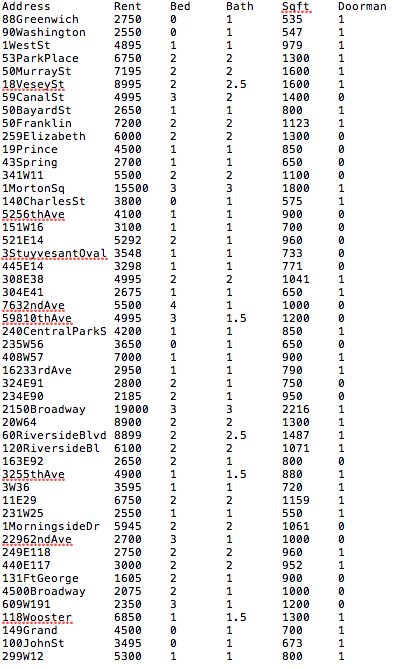
\includegraphics[scale=0.6]{newdata}
\end{center}
\end{document}